\documentclass[a4paper,12pt]{report}

\usepackage{rapportutc}
\usepackage{setspace}
\usepackage[final]{pdfpages}

\title{\textbf{Rapport de période d'apprentissage} \\Troisième année}
\author{Thomas \bsc{kieffer}}
\date{\today}

\uv{PAE03}
\semestre{A15 - P16}
\branche{Génie Informatique}
\filiere{Ingénierie des}
\specialite{Systèmes d'Information}

\suiveurutc{Vincent \bsc{fremont}}
\suiveurets{Guillaume \bsc{gesquière}}
\entreprise{Vallourec Tubes France}
\logoets{
\includegraphics[width=6cm]{img/logoets.jpg}}
\lieustage{CTIV Saint-Saulve, France}


\begin{document}
\stagepdtitre
\restoregeometry
\onehalfspacing
\tableofcontents

\chapter{Remerciements}
\paragraph{}
Avant de commencer ce rapport je tiens à remercier les personnes avec qui j'ai travaillé au cours de cette dernière année : Romain, Rémi, Jérémy, Aurélie, Klaus et Andreas de l'équipe \textit{Lan \& Cabling}, Frédéric et Benjamin de l'équipe \textit{ToIP, Wan \& Global Services}, Stéphane, Jérôme et Maxime de l'équipe \textit{Internet Security}, pour toutes le connaissances qu'ils m'ont apportées. Et bien évidemment Guillaume pour sa disponibilité et son écoute.

\paragraph{}
Merci aussi à tous mes collègues du CTIV, notamment les équipes \textit{Server}, \textit{Workstation}, \textit{Windows}, \textit{Linux}, pour leurs enseignements.

\paragraph{}
Merci également aux responsables apprentissage de l'UTC  ainsi qu'à mon tuteur, M. Fremont, qui ont su être disponibles et de bon conseil.

\chapter{Introduction}
\section{Objectifs du rapport}
Ce rapport représente la clôture de ma troisième (et dernière) année d'apprentissage, une nouvelle année riche en changements et en enseignements variées. Je présenterai les différentes activités que j'ai été amené à réaliser au cours de cette période en expliquant leur intérêt dans ma formation. Ce document va également me permettre de prendre le recul nécessaire à l'analyse des ces trois années passées au sein de Vallourec, de faire une mise au point sur mes acquis, mes compétences et ma capacité à exercer le métier auquel j'ai été formé. Je reviendrai également sur ma vision du métier d'ingénieur et mon aptitude à l'exercer.

\section{Contexte d'entreprise}
Cette section a pour objectif de remettre brièvement le lecteur dans le contexte de Vallourec afin de mieux comprendre mon environnement de travail. Ce contexte ayant peu évolué en comparaison de l'année précédente, les idées sont très semblables à celles exprimées en introduction de mon rapport de l'année précédente.

\paragraph{}
Le groupe Vallourec fournit des solutions tubulaires pour de nombreuses applications industrielles. 
Les deux tiers du chiffre d'affaires annuel de Vallourec proviennent du marché du pétrole et du gaz. Par conséquent, la santé de l'entreprise en est très dépendante. L pris très faibles du baril de pétrole au cours de cette année ont fortement impacté les clients de Vallourec qui ont ralenti leur rythme de commandes de tubes. L'activité des usines a donc continué à ralentir, ce qui a conduit à des périodes de chômage partiel voire à der fermetures de lignes de production. Comme ultime conséquence le plan Vallourec a annoncé début 2016 un plan social visant à réduire d'au moins un tiers le nombre de postes en France. Les fonctions support telles que l'informatique on également souffert du ralentissement de l'activité des usines : celles-ci n'ayant plus moyen de financer les projets d'évolution, ceux-ci se retrouvent bloqués.

\section{L'équipe, rôle et enjeux}
Mon poste de travail est basé au Centre de Traitement de l'Information de Vallourec (CTIV), lui-même localisé à Saint-Saulve près de Valenciennes. Le CTIV est le cœur informatique de Vallourec sur l'Europe, l'Afrique et le Moyen-Orient (\textit{EMEA}), c'est ici que sont prises les décisions les plus importantes concernant l'informatique, et que sont gérés les incidents, les problèmes et les évolutions d'architecture.
\paragraph{}
Au sein du département \textit{Infrastructure}, j'appartiens à l'équipe réseau du CTIV, cette équipe est elle même subdivisée en trois sous-équipes :
\begin{itemize}
\item L'équipe Internet Sécurité qui gère les communications entre le réseau interne Vallourec et l'extérieur, ce qui inclut les accès internet et les systèmes de protection tels que les pare-feu.
\item L'équipe ToIP, WAN \& Global Services est responsable de l'infrastructure de téléphonie sur IP ainsi que des connexions inter-sites du réseau Vallourec.
\item L'équipe LAN \& Cabling, à laquelle j'appartiens, est en charge des connexion réseau intra-sites, de leur maintenance et de leur évolution.
\end{itemize}

\paragraph{}
De même que la seconde année, ma mission en entreprise a été confondue à celle de l'équipe réseau, j'ai été amené à travailler sur tout les missions qui ont été confiées aux membres de l'équipe. Le réseau informatique est essentiel pour l'entreprise, toutes les communications entre les employés y transitent. Il est d'autant plus important au CTIV puis qu'il permet la communication entre les serveurs, les systèmes de sécurité et leurs administrateurs.

\section{Bilan de l'année 2}
Au terme de la seconde année d'apprentissage, je tirai un bilan très positif de ma progression : j'avais acquis de nombreuses connaissances techniques qui me permettaient de prendre en charge la grande majorité des incidents qui survenaient soumis à l'équipe ce qui m'a permis d'être beaucoup plus autonome. Au delà du plan technique, j'avais également acquis une meilleur aisance relationnelle qui me permettait d'échanger plus facilement et efficacement avec mes collègues.

\section{Objectifs et souhaits} %de moi perso
Au début de cette troisième année, j'espérais progresser aussi vite qu'au cours de la seconde année. Je souhaitais augmenter encore mes compétences techniques mais également monter en compétences sur un aspect plus organisationnel, gestion de tâches/projets et prendre plus de responsabilités que je n'en avais lors de l'année précédente.\\
Un des points qui me tenait à cœur au début de cette troisième année était de m'éloigner progressivement des tâches de maintenance opérationnelle pour me consacrer à des projets d'évolutions du parc. Je souhaitais également avoir la possibilité de prendre en charge un projet afin d'en découvrir les aspects et les méthodes de gestion.

%AJOUTER DES CHOSES ICI

\chapter{Activités réalisées}
Cette partie va me permette de décrire les activités réalisées au cours de cette dernière année. Pour chacune d'entre elles, en plus d'expliquer en qui elles ont consisté, je tenterai d'analyser l'intérêt que ces tâches et projets ont eu pour ma formation, les différentes enseignements que j'en ai tiré.
\paragraph{}
Au cours de cette année, j'ai été amené à contribuer à de nombreux projets et tâches. Néanmoins, au delà de la maintenance opérationnelle effectuée au quotidien, la grande majorité de ces tâches s'inscrivaient dans des grandes catégories : Sécurisation du réseau, supervision \& gestion des équipements, architecture WiFi. Du fait que ces sujets m'intéressaient particulièrement, je m'y suis auto-formé lors des périodes mois chargées ce qui m'a permis d'acquérir des compétences très solides sur ces sujets et ainsi de devenir très performant. C'était donc les sujets qui m'étaient confiés en priorité.

\section{Maintenance opérationnelle}
De même que l'année précédente, la maintenance opérationnelle (appelée \textit{run}) a occupé une partie importante de mon temps au cours de cette année. Pour rappel, le \textit{run} regroupe un grand nombre de tâches telles que la configuration d'équipements, le déplacement sur site pour changer un appareil défectueux, l'application de mises à jour sur les équipements en production, la résolution d'incidents, etc ... En résumé, il s'agit de toutes les actions que l'équipe doit entreprendre pour assurer le fonctionnement du réseau informatique au quotidien et pour que les utilisateurs puissent travailler. Comme les années précédentes je ne pourrai pas décrire toutes les tâches réalisées dans le cadre du \textit{run}. Dans les paragraphes suivants, je présenterai les tâches et aspects les plus intéressants du \textit{run} sur lesquels j'ai travaillé au cours de cette année.

\subsection{Support client}
Le support client est le caractère principal du \textit{run}. En ce qui me concerne, cet aspect a peu changé par rapport aux années précédentes. J'ai été en contact avec les équipes informatiques locales (sur les sites Vallourec distants) qui sont les points de remontées des incidents qui surviennent sur leurs sites. Ceux-ci nous contactent alors pour soumettre ces incidents afin de mettre en place une solution.
\paragraph{}
J'ai néanmoins acquis une aisance supplémentaire par rapport à la prise ne charge de ces incidents : pour la plupart des appels reçus, j'ai été capable de déterminer l'origine du problème ou, à défaut de mettre en place un processus de diagnostic permettant de déterminer cette cause. Par la suite, j'ai également été capable de proposer puis de mettre en production des solutions de résolution ou de contournement pour ces problèmes.
\paragraph{}
L'exemple typique pour illustrer ces propos est le cas de la défaillance d'un équipement (chose qui arrive fréquemment). Dans ce cas, il faut prendre en charge l'incident le plus vite possible afin de rétablir le service au client. Grâce à l'expérience acquise au contact d'incidents de ce type et à mes connaissances du fonctionnement du réseau, je suis capable d'identifier rapidement l'origine de la panne : défaut de courant, défaut de câble, mise en sécurité d'un appareil, défaut de configuration... De plus dans chaque cas, je suis apte à mettre en place une solution de réparation efficace.
\paragraph{}
Une nouveauté pour moi cette année a été la gestion d'incidents avec l'aide de nos fournisseurs. En effet, en plus de l'achat des équipements, Vallourec loue un service de maintenance pour ces appareils chez un de nos fournisseurs. Ces contrats agissent comme une assurance contre les défaillances des appareils en permettant de demander un remplacement en cas de problème matériel et le prêt d'une expertise technique en cas de problème de configuration et/ou d'architecture. Lors de la gestion de certains incidents, j'ai donc été amené à prendre contact et gérer les échanges avec ces fournisseurs pour trouver une solution.\\
Ce nouvel aspect m'a permis de progresser sur plusieurs points : premièrement sur les échanges avec des employés d'entreprises extérieures et deuxièmement sur des notions techniques que je ne connaissais pas, expliqués par des experts en la matière.

\subsection{Remplacement d'équipements en fin de vie} % + d'autonomie
Cette partie fait suite au projet de remplacement des appareils en fin de vie auquel j'avais participé au début de 2015. Pour rappel : au bout de quelques années, les équipements réseau ne sont plus mis à jour par leur fabricant (Cisco dans le cas de Vallourec). Il peu alors arriver que les derniers logiciels contiennent des failles de sécurité qui puissent alors être exploitées à des fins malveillantes. Pour éviter cette éventualité, les appareils qui ne sont plus supportés (en fin de vie) doivent être remplacés.
\paragraph{}
Connaissant bien le sujet de ce projet, celui-ci a été plus intéressant pour son aspect organisationnel que pour son aspect technique. Pour la préparation de l'intervention, j'ai pu profiter d'une grande liberté pour configurer les appareils et l'organisation de l'intervention (préparation du déplacement, planification des étapes, établissement des procédures de test).
\paragraph{}
Cette tâche qui s'inclut dans un projet plus large mais qui fait quand même partie des tâches de maintenance a été une expérience intéressante  car elle m'a permis d'apprendre à gérer une intervention avec impact comme celle de façon à ce que tout se déroule correctement.

\subsection{Diagnostic pont Wifi} \label{pt-wifi}
Cette section fait écho au projet de mise en place d'un pont WiFi, détaillé dans la partie \ref{pont_wifi}. Peu de temps après la mise en production de cette infrastructure, les utilisateurs ont remonté à l'équipe des gros problèmes d'instabilité de la connexion qui fonctionnait très mal. Ayant réalisé les tests et la configuration du projet, j'ai naturellement pris en charge le problème.
\paragraph{}
Après de nombreuses recherches pour établir un diagnostic et assisté de mes collègues, nous n'avons pas pu trouver la cause du problème. Il a alors été décidé d'ouvrir un incident chez notre fournisseur (comme expliqué précédemment) afin d'obtenir une assistance technique. J'ai donc pris en charge les échanges avec les experts ainsi que la communication avec les utilisateurs en usine.
\paragraph{}
Après de nombreux échanges avec les experts techniques et des discussions sur la configuration des appareils, je me suis replongé dans le problème en établissant une procédure de diagnostic plus rigoureuse plutôt que de me reposer sur l'expertise du fournisseur. Après récupération des informations remontées par les les équipements et analyse approfondie en m'appuyant sur des documentations, je suis parvenu à identifier l'origine du problème. Les déconnexions étaient dues à des perturbations du signal WiFi par des ondes radar émises à proximité. J'ai donc pu déterminer comment mettre en place une solution : il fallait changer la fréquence de communication du pont WiFi pour éviter les perturbations. Après plusieurs tests en périodes creuses, la nouvelle la fréquence a été changée sur le pont qui s'est stabilisé et a permis aux utilisateurs de retrouver une connexion réseau fonctionnelle.
\paragraph{}
Le travail sur le diagnostic du pont WiFi m'a particulièrement intéressé. Au delà de la satisfaction d'être parvenu à résoudre le problème, j'ai appris que mettre en place une procédure de diagnostic rigoureuse permettait d'organiser les idées et d'éliminer des causes possibles pour déterminer la véritable cause. J'ignorais également que les ondes radar pouvaient perturber le fonctionnement du réseau WiFi.

\subsection{Recul sur le \textit{run}}
Avec le recul, je remarque que les tâches de maintenance opérationnelle on peu changé depuis l'année précédente et que celles-ci ont occupé la majorité de mon temps. Grâce à l'expérience acquise les années précédentes, j'ai pu être beaucoup plus efficace dans la prise en charge et la gestion d'incidents. Cet aspect du travail est très gratifiant, j'apprécie apporter mon aide à mes collègues et clients et entendre leur satisfaction.
\paragraph{}
En revanche, ayant fait de grands progrès auparavant, ces tâches m'ont de moins en moins intéressé au fil du temps. De plus, avec le ralentissement de l'activité des usines, le nombre de tâches de maintenance à réaliser a considérablement diminué, résultant en des périodes d'oisiveté particulièrement frustrantes.

\section{Sécurisation du réseau}
Comme évoqué précédemment, un de mes grands axes de travail cette année a été la sécurisation du réseau. Je me suis beaucoup investi dans cette thématique car c'est un point qui m'intéressa particulièrement. Je travail que je regroupe dans cette section est très varié : il s'agit à la fois de tâches réalisées dans le cadre de l'équipe mais également en assistance de l'équipe \textit{internet security}.
\subsection{Enjeux}
L'enjeu de la sécurisation du réseau est évident. Dans ce cas, l'équipe étant chargée des réseaux locaux, j'ai avant tout été amené à travailler sur la sécurisation des accès au réseau en interne, c'est à dire la connexion par câble et en WiFi. 
\subsection{Cisco ACS}
\begin{wrapfigure}{r}{3.8cm}
\centering
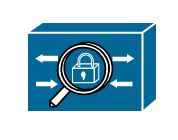
\includegraphics[scale=1]{../rapport_photos/acs_logo.JPG} 
\end{wrapfigure}
Le serveur ACS (symbolisé par le logo ci-contre)  est une solution d'authentification centralisée fournie par Cisco dont l'objectif est de permettre de gérer toutes les authentification sur le réseau en un point unique. En utilisant un hiérarchie de "magasins d'identités" (\textit{Active Directory}, liste d'adresses MAC, certificats ...), de règles d'identification et de politiques d'accès, le serveur ACS permet de gérer de façon très fine les accès de toutes les personnes au réseau mais également aux équipements. Le fonctionnement de cette plateforme repose sur deux protocoles distincts :
\begin{itemize}
\item
Le protocole TACACS (\textit{Terminal Access Controller Access-Control System})est un protocole propriétaire Cisco, il permet de gérer l'authentification des administrateurs sur les équipements réseau. Les différents magasins d'identités et règles d'authentification permettent de n'autoriser que certaines personnes à accéder à certains équipements. Ce protocole permet donc de gérer les accès des administrateurs aux équipements depuis le serveur uniquement.
\item
Le protocole RADIUS (\textit{Remote Authentication Dial-In User Service}) est un protocole standard qui permet de gérer les accès utilisateurs au réseau. Sa grande flexibilité permet de gérer les requêtes provenant de nombreuses sources, aussi bien filaire que sans-fil, tout en restant rapide et efficace.
\end{itemize}
\paragraph{}
C'est donc sur ces deux protocoles et sur le serveur ACS que je me suis basé pour les différentes tâches de sécurisation du réseau que j'ai été amené à réaliser.

\subsection{Projet \textit{Common ACS}}
%Ajouter les présentations et exposés et schémas (annexe aussi)
Le projet Common ACS devait être le projet le plus imposant qui m'ai été confié au cours de mon apprentissage et qui aurait du occuper une partie conséquente de mon temps sur les mois d'avril et mai 2016. Ayant acquis précédemment de bonnes connaissances sur le fonctionnement du serveur ACS, ce projet m'a été confié. J'avais donc en charge l'établissement de l'architecture et sa mise en production.
\subsubsection{Contexte}
Suite au rapprochement des équipes réseau française et allemande en 2014, la mutualisation des infrastructures et des outils avait commencé en 2015. Après avoir remarqué que les architectures réseau étaient très semblables des deux côtés de frontière, il a été décidé de les rassembler pour arriver à une architecture globale et commune. Il en a été de même pour l'ACS, avec deux serveurs de chaque côté de la frontière, il a été jugé utile de les combiner.
\subsubsection{Objectifs}
L'objectif principal du projet était donc de regrouper les systèmes d'authentification de France et d'Allemagne afin de réorganiser les flux d'authentification et de pouvoir gérer l'ensemble du parc de l'équipe depuis un point d'entrée unique. Les objectifs secondaires de ce projet étaient nombreux : au delà de l'aspect symbolique du rapprochement France-Allemagne, la nouvelle architecture allait permettre un service plus efficace et surtout secouru puisque les systèmes français et allemands devaient prendre le relais l'un de l'autre en cas de défaillance.
\subsubsection{Architecture}
La première étape de ce projet a été de définir l'architecture cible. Pour cela, j'ai mis en place et suivi les étapes suivantes :

\paragraph*{Inventaire du matériel et étude de l'architecture existante}
J'ai commencé par étudier la façon dont étaient conçues les deux architectures ACS. Connaissant bien le fonctionnement du serveur français, cette étape s'est déroulée rapidement : l'ACS est constitué de deux serveurs applicatifs fonctionnant sur deux machines virtuelles séparées sur deux châssis hyperviseurs VMware (physiques) séparés. L'application ACS fonctionne donc en cluster : un serveur primaire et un secondaire capable de prendre le relais en cas de défaillance. L'architecture est identique du côté allemand, seule la configuration diffère du fait d'une approche des règles d'authentification différente. Cette première étape m'a permis d'avoir connaissance des équipements à ma disposition ainsi que de la configuration à reproduire dans le serveur final. J'ai également pu mettre en évidence une différence de version logicielle entre les serveur allemands et ceux en France, ce qui était gênant pour la suite du projet étant donné qu'il est impossible de monter un cluster de serveurs de versions (même mineures) différentes. Dès le départ, j'ai dû donc planifier la mise à jour des serveurs français.

\paragraph*{Étude des configurations recommandées par Cisco}
N'étant pas un expert en matière d'ACS, je me suis tourné vers les documentations proposées par Cisco afin de connaitre les \textit{Validated Designs} en matière d'architecture de serveurs ACS (autrement dit, les types d'architectures recommandés par le fabricant). Ces documents existent pour tous les produits Cisco et sont fréquemment utilisés par l'équipe dans le cas de conception de nouvelles architectures comme bases de réflexion. Cela permet de partir sur des bases saines et éprouvées. Dans le cas de l'ACS, ces documents préconisent de tirer profit de plusieurs serveurs à la fois afin de répartir la charge de travail. Il existe 3 rôles dans une architecture ACS : 
\begin{itemize}
\item
Le serveur \textbf{primaire} est le point d'entrée (unique) d'administration. Sa configuration est répliquée sur les serveurs secondaires.
\item
Les autres serveurs sont \textbf{secondaires} : ils reçoivent la configuration du primaire et répondent aux requêtes des appareils clients.
\item
Rôle à cumuler avec l'un des deux précédents, le \textbf{collecteur de log} récupère les évènements qui surviennent sur tous les membres de l'architecture pour les rendre consultables. Les \textit{validated designs} conseillent de ne pas affecter le rôle de collecteur à un serveur réalisant l'authentification afin de répartir la charge.
\end{itemize}  
A l'issue de cette étape, j'avais une idée bien plus précise des configurations que je pouvais mettre en place à partir des quatre serveurs à ma disposition.


\paragraph*{Conception d'architectures suivant les configurations recommandées}
Par la suite je me suis occupé d'adapter les \textit{validated designs} à l'environnement de Vallourec et surtout aux différents appareils qui doivent se connecter au serveur ACS (clients, contrôleurs WiFi, switchs, routeurs, serveurs, applications...). Après réflexion et de nombreux schémas, j'ai jugé comme les plus intéressants les architectures présentées ci-dessous. Il est important de noter que le matériel physique était conservé : je suis parti sur une base de 4 serveurs ACS avec pour objectif de les monter en cluster afin d'obtenir un unique serveur virtuel.
\\

\textbf{Première proposition :} un serveur primaire et un secondaire dans un pays et deux secondaires dans l'autre. Indépendamment des protocoles, tous les appareils s'authentifient sur un des secondaires dans leurs pays respectifs, le collecteur de logs est le secondaire qui ne sert pas d'authentificateur. L'intérêt de cette architecture est qu'elle est très semblable à l'ancienne architecture et aurait nécessité très peu de changements sur les appareils clients, en revanche, elle ne respecte pas tous les principes des \textit{validated designs} car il n'y a pas de distinction entre les types d'appareils.
\begin{figure}[h]
\centering
\includegraphics[scale=0.5]{../rapport_photos/ACS1.png} 
\end{figure}

\textbf{Seconde proposition :} authentification des appareils TACACS dans un pays et des appareils RADIUS dans l'autre, le collecteur de logs est le secondaire qui ne sert pas d'authentificateur. Cette architecture respecte les \textit{validated designs}.
\begin{figure}[h]
\centering
\includegraphics[scale=0.5]{../rapport_photos/ACS2.png} 
\end{figure}

\textbf{Troisième proposition :} le serveur primaire et point d'entrée ne sert pas de serveur d'authentification mais de collecteur. Les trois autres servent pour authentifier respectivement les appareils TACACS, les appareils RADIUS qui se présentent en WiFi et les appareils RADIUS qui se présentent en filaire (voir \ref{802.1x}). Cette architecture respecte les \textit{validated designs} et présente en plus l'avantage d'anticiper l'évolution du réseau qui prévoit d'étendre l'authentification en filaire à toute la France et l'Allemagne. Dans le cas de cette architecture, les trois serveurs authentificateurs se secourent mutuellement, dans le cas de la perte de connexion, les appareils d'un pays peuvent se rabattre sur le (ou les) serveur(s) dans le pays.
\begin{figure}[h]
\centering
\includegraphics[scale=0.5]{../rapport_photos/ACS3.png}
\end{figure}

\paragraph*{Présentation à l'équipe et prise de décision}
Une fois les concepts d'architecture préparés, j'ai profité d'une réunion d'équipe franco-allemande pour les présenter à mes collègues et recueillir leurs avis. après la présentation, les avis étant partagés, nous avons discuté et argumenté pour trouver un compromis. Au final, c'est la troisième option qui a été retenue par l'équipe comme version finale de l'architecture.

\paragraph*{Préparation de la configuration commune}
L'étape finale de la conception concernait la configuration des serveurs. En effet, pour avoir un unique serveur, il fallait unifier les configuration utilisées en Allemagne et en France. Les serveurs ayant la même utilité dans les deux pays il m'a fallu choisir une des deux "philosophies de configuration" et adapter l'autre à la première en utilisant les mêmes règles. Les magasins d'identité évoqués précédemment sont les mêmes pour toute la zone EMEA (l'\textit{Active Directory} notamment), de ce fait il n'était pas nécessaire de reconfigurer des magasins supplémentaires.

\subsubsection{Tests et procédures}
Après la conception du nouveau système il me fallait préparer la migration en elle même, c'est à dire le scénario (les étapes) de migration ainsi que les tests à réaliser pour valider le bon fonctionnement.
\paragraph{}
Le point critique était de mettre en place l'architecture choisie sans interrompre le service d'authentification qui aurait privé les utilisateurs de connexion réseau sur tous les sites français et/ou allemands. J'ai dû donc prêter une attention particulière à la procédure de mise en production et anticiper les conséquences de chacune des étapes afin d'éviter toute coupure intempestive.
\paragraph{}
Je n'ai en revanche pas préparé le protocole de test après déploiement car le projet à été mis en suspens à ce moment.

\subsubsection{Contraintes techniques}
En effet, lors de la préparation de l'étape préliminaire de mise à jour des serveurs français, après avoir étudié les procédures de mise à jour  fournies par Cisco, je me suis aperçu que les nouvelles versions du logiciel ACS nécessitaient une version spécifique de l'hyperviseur VMware sur lequel il était installé. Sans rentrer dans les détails complexes, il s'est avéré que la version VMware installée était inférieure à la version requise. Après discussion avec les équipes en charge des châssis, j'ai pris que les hyperviseurs de production ne seraient mis à jour qu'à la fin de l'année car la procédure était complexe à suivre et très impactante pour de nombreux serveurs de production. Le projet \textit{Common ACS} a donc été suspendu jusqu'à cette mise à jour essentielle. 

\subsubsection{Résultats}
La suspension de ce projet a été une grande déception car je m'y suis véritablement investi. Malgré tout, ce projet a été très enrichissant et je pense en avoir réalisé la partie la plus intéressante. J'ai non seulement découvert un aspect technique que je connaissais peu, mais j'ai aussi pu me pencher sur une véritable problématique demandant de la réflexion et une bonne préparation. D'autant plus que ce travail n'est pas perdu, il servira de base à mes collègues pour terminer le projet une fois la mise à jour effectuée.
\paragraph{}
Sur le plan personnel ce projet a également été valorisant car mon implication a été remarquée : mon équipe a souligné la qualité des documents produits ainsi que la clarté de mes présentations et explications.

\subsection{Projet 802.1X} \label{802.1x} %machines + iphones
Le projet 802.1X a également été un projet qui m'a beaucoup intéressé au cours de cette année. A mon grand regret et malgré mes demandes, je n'ai pas été impliqué dans la réalisation de ce projet. J'ai néanmoins pu suivre son avancement en assistant au travail de mes collègues et en réalisant quelques tests à côté afin e comprendre les techniques mises en jeu.
\subsubsection{La norme 802.1X}
La norme 802.1X est un protocole d'authentification des utilisateurs pour un accès réseau. Elle regroupe un grand nombre de mécanismes et est adaptable à tout type de réseau. Le schéma de fonctionnement classique du 802.1X est composé d'un appareil client (ex: un PC), d'un appareil authentificateur, membre du réseau, sur lequel le client se connecte (un switch), un serveur d'authentification (Cisco ACS) qui va vérifier l'identité du client (auprès d'un répertoire d'entreprise par exemple) avant lui donner ou non l'accès au réseau.
\subsubsection{Objectif du projet}
L'objectif du projet en question était de mettre en place la norme 802.1X sur le réseau filaire du CTIV afin de le rendre sécurisé. Dans ce cas, il avait été décidé de réaliser l'authentification de l'appareil client à l'aide de certificats et non par identifiants comme réalisé pour le WIFi.
\subsubsection{Reprise d'activité}
J'ai été amené à intervenir sur ce projet dans le cadre de la reprise d'activité le lendemain de la mise en place des règles d'authentification. Suite à plusieurs problèmes, de nombreux postes clients n'avaient pas réussi à installer leurs certificats, il se voyaient alors interdire l'accès au réseau. Du fait de mon expérience avec le serveur Cisco ACS, j'ai été apte à diagnostiquer très rapidement les connexions refusées et à proposer des solutions de contournement aux utilisateurs.
\subsubsection{Résultats et enseignements}
Personnellement, mon suivi du projet et contribution à la reprise d'activité m'ont permis de comprendre le fonctionnement du mécanisme 802.1X, norme très importante dans le domaine de la sécurisation du réseau.

\subsection{Résultats}%apports personnels et pour l'entreprise
Cet axe de travail que j'ai retrouvé tout au long de cette année a été pour moi une thématique très intéressante : j'ai développé un très grand intérêt pour la sécurisation des accès réseaux. Les techniques et méthodologies mises en place pour obtenir un réseau sûr sont multiples. J'en suis venu à m'intéresser de près à ces techniques notamment à la cryptographie qui sert lors des authentifications fortes (clés privées/publiques, cryptage des communications, échange de clés, signature de certificats ...), cet aspect m'a véritablement passionné.
\paragraph{}
Au delà de cet aspect, j'ai appris le fonctionnement des protocoles et des technologies utilisées pour sécuriser le réseau, ce qui m'a permis de gagner en autonomie lors du diagnostic d'incidents d'accès et d'authentification.
\paragraph{}
Du point de vue de l'entreprise, je suis devenu un élément clé pour la mise en place et le débogage de systèmes d'authentification basés sur l'ACS Cisco.

\section{Supervision et gestion des équipements}
Cette partie fait suite au projet supervision mis en place dès 2014 et qui avait pour but de renforcer la supervision des équipements et la d'améliorer la qualité des informations remontées.
\paragraph{}
Pour rappel, la supervision du réseau est une partie importante du travail de surveillance du réseau. Le terme \textbf{supervision} regroupe deux aspects : \textit{un mécanisme d'alertes} qui permet d'informer les administrateurs de défaillances sur le réseau, notamment lors de la perte de connexion avec un appareil; et \textit{la gestion du parc (management)} qui permet de conserver un inventaire des appareils en production, leurs caractéristiques, leurs configurations ... Ces deux aspects seront parfois distingués par la suite.

\subsection{Objectifs et enjeux}
Au cours de cette dernière année d'apprentissage, le projet supervision a évolué avec le changement de contexte. Suite au rapprochement France-Allemagne, il avait été décidé que l'équipe utiliserait des outils communs des deux côté de la frontière.

\subsection{Étude de différents outils}
Dans l'objectif de trouver un outil commun à l'équipe unifiée, un appel d'offre avait été lancé à nos fournisseur afin que l'on soit orientés vers des outils correspondant le mieux à nos besoins. Suite à des retards dans le planning et dans les réponses des fournisseurs, il s'est avéré que le délai restant pour choisir un outil était très court avant la clôture des budgets pour l'année.
\paragraph{}
L'équipe m'a donc confié la tâche de réaliser une étude rapide (moins de deux semaines) de plusieurs outils du marché afin de tester leurs performances. En partant des critères qui avaient été transmis aux fournisseurs, j'ai recherché, installé et testé plusieurs logiciels.
\paragraph{}
Sur les conseils d'une autre équipe, nous nous sommes également penchés sur les outils proposés par la société Infoblox et notamment sont logiciel de supervision : \textit{Network Automation}. Avec la rencontre d'un ingénieur avant-vente et l'installation d'un plateforme de test sur notre réseau, nous avons pu avoir un bon aperçu des performances de cet outil.

\subsection{Résultats}
%Distinguer aletring et monitoring ?
Au final, parmi tous les outils évalués, c'est celui de la société Infoblox qui a été retenu comme le plus apte à remplacer les outils actuels sur la partie \textit{management} de la supervision. Concernant  les alertes, il a été décidé de conserver l'outil allemand (Solarwinds) afin de conserver au moins un outil connu et fiable pour la partie la plus importante de la supervision.

\subsection{Rapports de performance}
A l'aide du nouvel outil d'Infoblox (que j'appellerai NetMRI par la suite), j'ai pu mettre en place des routines de vérification du bon fonctionnement du réseau, que ce soit au niveau de la configuration et des performances. Les fonctionnalités du logiciel permettent de définir des règles qui vont être comparées à l'état de l'équipement en production, ces règles sont assemblées en politiques qui elles sont déployées sur les appareils. Ces politiques sont alors capables de rendre compte de l'exactitude des configurations et des bonnes performances des appareils.

\subsection{Automatisation des tâches}
Une des fonctionnalités les plus intéressantes de \textit{Network automation} est sa capacité à se connecter aux équipements du réseau suivants des scripts écrits dans un langage propriétaire. Dès la mise en place de l'environnement de test, j'ai remarqué le potentiel d'une telle fonctionnalité : automatiser et paralléliser les tâches de configuration récurrentes sur les équipements.
\paragraph{}
Une fois le logiciel mis en production, je me suis documenté afin de comprendre comment automatiser certaines tâches sur le réseau et comment fonctionnait ce langage propriétaire. J'ai également commencé à identifier les tâches de contrôle et de configuration récurrentes et chronophages afin de trouver un moyen de les automatiser.
\paragraph{} 
La procédure la plus utile que je suis parvenu à mettre en place concerne le déploiement du réseau d'isolement sur les switchs. Pour des raisons de sécurité, les prises réseau qui desservent les bureaux et usines doivent être positionnées dans un sous-réseau d'isolement par défaut. Cela a pour effet d'empêcher un appareil non autorisé d'accéder au réseau en se connectant sur une prise libre. L'inconvénient de cette méthodologie de sécurité et que toutes les manipulations doivent être déployées à la main, en ligne de commande après de multiples vérifications, ce qui est très gourmand en temps. L'intérêt d'automatiser cette tâche était évident : en plus d'accélérer le traitement, il n'est plus nécessaire de monopoliser une personne pour gérer les opérations.
\paragraph{}
Le développement du script a été complexe et m'a occupé sur quelques jours avant que j'obtienne un fonctionnement efficace et fiable. Après plusieurs tests sur des séries d'équipements de plus en plus importantes, j'ai pu conclure que celui-ci était utilisable sur la production. Les résultats ont été impressionnants : il fallait entre 3 et 4 heures à un membre de l'équipe pour traiter une vingtaine d'appareils, le script pouvant fonctionner sur jusqu'à 20 appareils en même temps, les traite de façon totalement autonome en moins de 10 minutes. Ceci représente un gain de temps considérable pour l'équipe.
\paragraph{}
J'ai apprécié travailler sur cette fonctionnalité qui m'a permis de me pencher sur une problématique différente de celles rencontrées au quotidien et qui a fait prendre conscience à l'équipe du potentiel de la solution d'Infoblox en matière d'automatisation des tâches. Par la suite, j'ai continué à travailler sur d'autres scripts, notamment sur des mécanismes permettant de vérifier les configurations des switchs et de les corriger en cas de problème.

\section{Architectures WiFi contrôlées}
% FAIRE DES SCHEMAS !!!
\subsection{Définition, contexte et objectifs}
Au cours de cette troisième année, la seconde thématique qui m'a beaucoup intéressé est la conception/mise en place d'architectures WiFi contrôlées. Une architecture contrôlée est basée sur un serveur central appelé \textit{contrôleur} auquel sont associées des bornes WiFi. Ces bornes sont les points d'entrée des clients WiFi, elles diffusent les réseaux configurés. Cette configuration est réalisée depuis le contrôleur qui est chargé de la faire appliquer sur les bornes qui lui sont associées. L'intérêt de cette architecture est qu'elle permet une configuration par interface graphique et en un point unique. Elle s'oppose à l'architecture "lourde" dans laquelle les bornes sont indépendantes et doivent être configurées manuellement en ligne de commande ce qui est beaucoup plus chronophage.
\paragraph{}
Pour comprendre l'intérêt des projets détaillés par la suite, il est nécessaire de comprendre les deux variantes de l'architecture contrôlée utilisées. La première est l'architecture centralisée standard (Figure \ref{wifi_standard} ) composée d'un contrôleur sur site auquel sont associées toutes les bornes du réseau local. Dans cette configuration, le trafic des clients sans-fil est transféré sur le réseau filaire et remonte jusqu'au contrôleur via un tunnel virtuel. ainsi, en sortie de la borne, les données sont encapsulées et sont indépendante du reste du trafic. Une fois arrivées au contrôleur, ces données sont traitées et renvoyées dans le sous-réseau adéquat vers leur destination. Ainsi, du point de vue du reste du réseau, un client WiFi sera perçu comme provenant du contrôleur.
\begin{figure}[h]
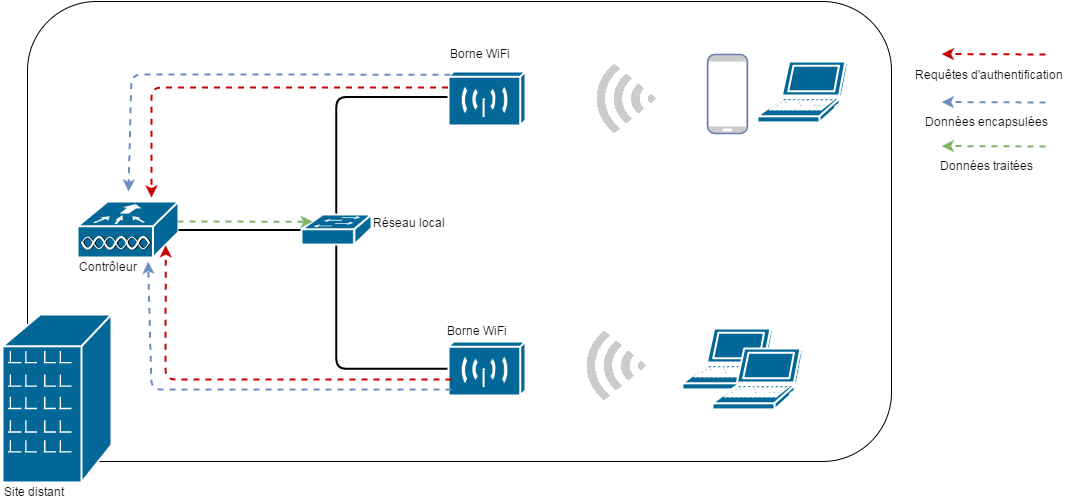
\includegraphics[scale=0.4]{../rapport_photos/wifi.png} 
\caption{Architecture contrôlée standard}
\label{wifi_standard}
\end{figure}

\paragraph{}
Les projets détaillés par la suite ont fait appel au mode \textbf{FlexConnect} de l'architecture contrôlée. Ce mode diffère du mode standard par le fait que les données ne remontent plus jusqu'au contrôleur mais sont envoyées dans le bon sous-réseau dès la sortie (filaire) de la borne (Figure \ref{wifi_flex}). Seuls les données de synchronisation et d'authentification sont envoyées au contrôleur c'est pourquoi ce dernier est nécessaire. En mode FlexConnect, si la borne perd la connexion avec le contrôleur, elle ne pourra plus accepter de nouvelles connexions mais celles déjà établies continueront de fonctionner. L'intérêt de ce mode est que le contrôleur n'est pas nécessairement sur le même réseau local que les bornes qu'il gère.
\begin{figure}[h]
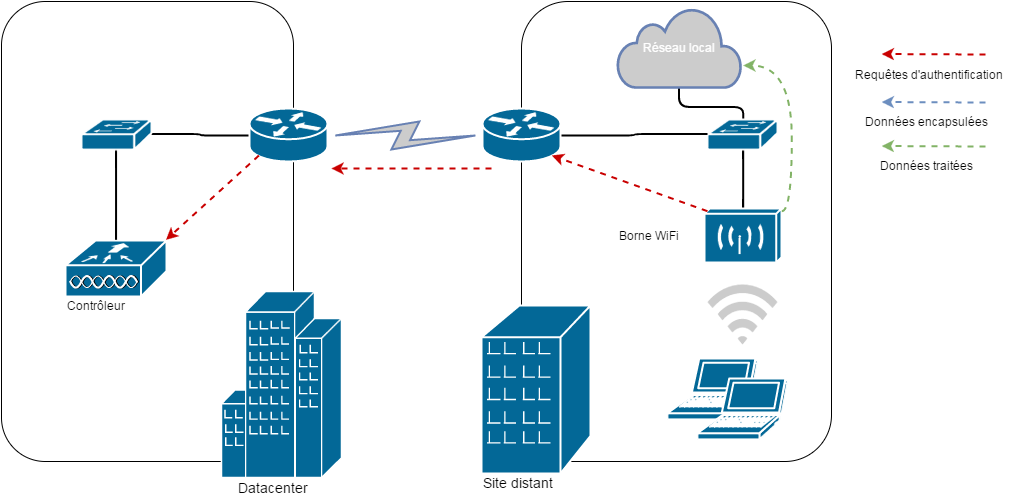
\includegraphics[scale=0.4]{../rapport_photos/wifi_flex.png} 
\caption{Architecture contrôlée FlexConnect}
\label{wifi_flex}
\end{figure}

\subsection{Préparation du contrôleur}\label{controleur}
Afin de pouvoir tester le mode FlexConnect, j'ai dû réutiliser un contrôleur de secours présent au CTIV. Je me suis donc chargé de désinstaller cet appareil et de préparer une nouvelle configuration. Le mode FlexConnect permet de mettre en place une architecture centralisée géographiquement, il a donc été décidé d'installer le contrôleur au datacenter pour qu'il soit facilement joignable depuis tous les sites. Une fois le contrôleur installé sur place et mis en marche, j'ai pu commencer à l'utiliser pour y mettre en place des nouveaux réseaux.

\subsection{Architecture contrôlée FlexConnect}
Cette section décrit le projet que j'ai réalisé au cours de l'été 2015. L'usine Vallourec de Maubeuge utilisait à l'époque une architecture lourde peu performante et qui n'était plus conforme aux règles de sécurité de l'entreprise. L'objectif était donc de reconfigurer entièrement cette architecture pour la transformer en architecture contrôlée FlexConnect.
\paragraph{}
Après avoir réalisé plusieurs tests au CTIV avec des bornes configurées en FlexConnect, j'ai préparé la migration des toutes le bornes de l'usine. La difficulté de cette opération était de faire passer les bornes du mode "lourd" au mode centralisé. Pour ce faire, il faut changer la version du système d'exploitation mais ceci occasionne sa réinitialisation. Habituellement, lors de ces opérations, il suffit de connecter un pc en direct à la borne pour y accéder en ligne de commande et lui renseigner l'adresse IP de son contrôleur. Dans ce cadre, les bornes étaient déjà installées dans l'usine donc certaines dans l'atelier à plusieurs mètres de hauteur et donc impossibles d'accès pour les configurer. Pour contourner ce problème, j'ai mis en place la transmission de l'adresse du contrôleur via le DHCP.
\paragraph{}
Une fois sur place pour réaliser l'intervention, je me suis occupé de mettre à jour les bornes une à une avec le nouveau système d'exploitation en vérifiant qu'il était bien fonctionnel avant de lancer la migration vers le contrôleur. Deux de ces bornes on connu des difficultés au redémarrage, l'une d'elles était facilement accessible, j'ai pu donc la configurer manuellement, l'autre était hors d'atteinte mais son comportement par défaut dans ce genre de cas m'a permis de la configurer à via le réseau. Au final, malgré ces difficultés, toutes les bornes ont changé de mode et se sont associées au contrôleur.
\paragraph{}
Ce projet a été très intéressant pour moi : il été le premier que j'ai pu gérer en autonomie, notamment lors de  l'intervention. J'ai non seulement pu travailler avec une technologie vraiment intéressante mais aussi planifier et réaliser une intervention. J'ai également dû faire appel à mes connaissance pour trouver des solutions aux problèmes rencontrés.

\subsection{Pont WiFi}\label{pont_wifi}
Ce projet fait suite à la demande d'une usine qui souhaitait alimenter en réseau un petit bâtiment très éloigné  des autres bâtiment de l'usine (environ 600 mètres), et donc du réseau déjà en place. Vu la situation économique difficile de l'entreprise, il avait été demandé que cette solution soit la moins coûteuse possible, d'autant plus que cette liaison ne desservirait que quelques appareils et ne nécessitait donc pas un débit élevé. Du fait de ces contraintes (distance et coût) il était impossible de mettre en place une connexion câblée ou fibrée. L'équipe a donc décidé de mettre en place un pont WiFi avec des bornes spéciales de grande puissance pour couvrir la distance.
Ce pont a été configuré et mis en place au milieu de l'année 2015 mais je n'y étais pas intervenu à l'époque.
\paragraph{}
Au cours des quelques mois suivant sa mise en place, le pont a connu de nombreux dysfonctionnements. Il avait été conçu et configuré à la main en ligne de commande avec des bornes "lourdes". Cette configuration est très complexe à réaliser de cette façon et encore plus difficile à diagnostiquer. C'est pourquoi l'équipe a pris la décision de reconcevoir le pont mais cette fois en mode contrôlé. Le contrôleur du datacenter ayant été installé depuis peu (voir \ref{controleur}) le pont a donc été conçu en mode FlexConnect, géré par le contrôleur au datacenter.
\paragraph{}
Du fait de mon expérience sur la configuration FlexConnect et mon grand intérêt pour le sujet cette tâche m'a été confiée. Comme pour les projets décrits précédemment j'ai commencé par me étudier la faisabilité de l'architecture en consultant des documentation, puis j'ai entrepris une phase de tests : à l'aide de deux bornes WiFi associées au contrôleur du datacenter, j'ai déployé les configurations recommandées. Sans succès dans un premier temps, j'ai fini par comprendre que l'établissement de la connexion prenait un certain temps. Une fois les paramètres affinées, j'ai présenté (de façon informelle) à l'équipe la procédure de mise en place qui a été validée.
\paragraph{}
J'ai donc enchaîné par la phase de mise en production : de la même façon que le projet précédent, j'ai mis à jour les bornes afin qu'elles passent en mode contrôlé et qu'elles s'associent avec le contrôleur du datacenter. Puis j'ai appliqué la configuration déterminée précédemment. A ce moment le pont s'est établi correctement et semblait fonctionner sans souci. Il s'est avéré par la suite qu'il subissait d'importantes déconnexions dues à des perturbations (voir partie \ref{pt-wifi}).

\section{Projets et missions transverses}
\subsection{Définition, objectifs et enjeux}
Cette partie va me permettre de détailler certaines tâches transverses que j'ai réalisées au cours de cette année. Je désigne comme tâche transverse une tâche qui m'a amené à travailler avec des membres des autres équipes.
\paragraph{}
Au cours de cette année, j'avais très à cœur de pouvoir m'intéresser davantage aux missions des équipes qui entourent (et utilisent) le réseau au quotidien, afin de comprendre leurs missions, leurs responsabilités et leur fonctionnement. Selon moi, c'est une qualité indispensable de l'ingénieur : il doit avoir la capacité de comprendre les personnes avec lesquelles il travaille et faire preuve d'empathie. Cette capacité est la clé d'un communication ouverte, claire et constructive qui est elle essentielle à un travail efficace.
\paragraph{}
Dans les parties à suivre, je détaillerai les tâches transverses que j'ai jugées les plus intéressantes et enrichissantes. Seule la démarche entrepris a un intérêt pour ce rapport, je ferai donc l'impasse sur les détails techniques dans la plupart des cas.

\subsection{Mise à jour des loadbalancers F5} \label{f5}
Le projet en question (porté par l'équipe \textit{Internet security})avais pour objectif de mettre à jour le logiciel des \textit{loadbalancers} situés au datacenter. Ces appareils sont utilisés pour répartir les flux de données sur les différents liens de sortie du datacenter, cette mise à jour concernait deux équipements : un primaire et un de secours. La problématique était qu'il fallait réaliser cette mise à jour sans interrompre la connexion des serveurs au datacenter, il était donc impossible de traiter les deux loadbalancers en même temps. Mon collègue s'est chargé de la planification et de l'organisation de l'intervention.
Pour ma part, j'étais chargé d'assister mon collègue et de réaliser l'intervention pour la partie réseau. 
\paragraph{} 
Les opérations à réaliser étaient simples mais présentaient un risque marqué. Dans ce cas, le risque était lié à l'impact potentiel : une perte de connexion avec les loadbalancers aurait induit une perte de connexion avec de nombreux serveurs de production du datacenter. Il fallait tout d'abord isoler le loadbalancer secondaire du réseau afin de pouvoir le mettre à jour. Cette étape n'avait aucun impact puisque l'appareil secondaire ne sert qu'en cas de défaillance du premier. Une fois la mise à jour terminée sur le secondaire, il fallait transférer les flux du primaire vers celui-ci. Opération qui ne nécessitait pas d'intervention réseau. De même que précédemment j'ai dû isoler le membre primaire afin qu'il soit mis à jour également. Pour finir, nous avons dû rétablir le système dans son état normal.
\paragraph{}
Au final, ce projet n'a pas été complexe à réaliser de mon côté puisque le travail le plus important était de la responsabilité de mon collègue. En revanche j'ai beaucoup appris sur la préparation d'une intervention présentant un risque fort. Cet apprentissage m'a servi quelques semaines plus tard lors de la suppression des firewalls PaloAlto.

\subsection{Suppression des firewalls PaloAlto} \label{palo}
Ce projet, également porté par l'équipe \textit{Internet security}, avait pour objectif de désaffecter les deux firewalls de marque PaloAlto installés au datacenter. A l'origine ces deux appareils servaient à analyser les flux transitant entre le réseau du datacenter, le WAN et les réseaux des entreprises partenaires. A la suite du renouvellement des équipements du datacenter l'année dernière, il avait été nécessaire de conserver des switchs supplémentaires pour permettre à ces firewalls de fonctionner.
\paragraph{}
L'équipe \textit{Internet security} s'est alors chargée de concevoir un nouveau schéma des flux afin de transférer l'analyse vers un châssis de firewalls Checkpoint plus récent et plus performant. Ceci permettait alors de retirer les appareils PaloAlto.
\paragraph{}
Comme précédemment, mon rôle a été de réaliser la partie réseau de l'intervention. L'idée était de faire modifier le chemin de passage des flux sur des liens physiques qui contournent les PaloAlto. Le risque ici était d'interrompre les connexion sur un des sous-réseaux qui transitait par les firewalls. Pour amoindrir ce risque, il nous a fallu préparer soigneusement l'intervention en envisageant tous les cas de figure afin d'anticiper les éventuels problèmes. L'intervention s'est réalisée en deux temps : 
\begin{itemize}
\item
Transfert des flux vers les firewalls Checkpoint. Côté réseau, j'ai du modifier le comportement des cœurs de réseau afin de faire transiter les flux vers les firewalls Checkpoint. A l'issue de cette partie, les flux étaient filtrés deux fois, il était donc possible de contourner les firewalls PaloAlto.
\item
Le contournement a été réalisé en utilisant des câbles déjà présents qui reliaient directement le réseau du datacenter aux anciens switchs qu'il avait fallu laisser en place. Sans rentrer dans les détails, j'ai dû reconfigurer les switchs afin de forcer les flux à transiter par ces liens de contournement.
\end{itemize}
\paragraph{}
Au final, l'intervention fut un succès avec des temps de coupure faibles et donc un impact très limité. L'objectif suivant était de retirer physiquement les switchs laissés pour le fonctionnement des PaloAlto. Mais cette étape n'a toujours pas été réalisée à l'heure où j'écris ces lignes. 
\paragraph{}
La réalisation de ce projet a été très satisfaisante pour moi car j'ai pu prendre en charge (et réussir) la partie réseau sans avoir besoin de l'aide de mes collègues. J'ai compris que mes compétences techniques associées à une bonne préparation me permettaient d'être sûr de réussir et m'ont permis de gagner en assurance.

\subsection{Projet \textit{DataCenter revamping}} \label{revamp}
Ce projet portait également sur l'infrastructure du datacenter : l'objectif était de sécuriser le réseau en faisant transiter tous les sous-réseaux via le châssis firewall Checkpoint afin de pouvoir analyser les flux. Au démarrage de ce projet j'avais peu de connaissances sur l'architecture logique du datacenter et surtout sur ses interconnexions avec les équipements des autres équipes. Afin de pouvoir réaliser la partie réseau des opérations de ce projet, il m'a fallu d'abord mieux comprendre cette architecture. J'ai donc étudié les documentations à ma disposition.
\paragraph{}
La migration d'un sous réseau était simple : quelques commandes à envoyer aux switchs pour réorienter les flux. La complexité de l'opération résidait dans le nombre de sous réseaux à migrer et dans la criticité de certains: les sous-réseaux de serveurs de production ne peuvent être interrompus qu'un très court instant.
\paragraph{}
De même que pour les opérations précédentes, le fait d'avoir bien étudié l'architecture précédente et d'avoir correctement préparer les commandes à envoyer m'a permis d'être sûr de moi lors de l'intervention qui s'est déroulée sans difficulté.

\subsection{Architecture du datatcenter}
Pour illustrer les 3 projets ci-dessus (\ref{f5}, \ref{palo}, \ref{revamp}), les figures \ref{fw_old} et \ref{fw_new} présentent l'architecture logique du datacenter avant et après les différentes interventions.
\begin{figure}
%\includegraphics[scale=0.5]{../rapport_photos/fw_old.png}
\caption{Ancienne architecture}
\label{fw_old}
\end{figure}
\begin{figure}
%\includegraphics[scale=0.5]{../rapport_photos/fw_new.png}
\caption{Nouvelle architecture}
\label{fw_new}
\end{figure}
La nouvelle architecture, en plus d'être simplifiée, permet d'avoir un contrôle plus précis des flux qui transitent dans le réseau. Elle facilite le travail de l'équipe \textit{Internet security} et a permis à l'équipe réseau de retirer les switchs qui n'étaient plus nécessaires.

%\subsection{Mise à jour des appareils de visioconférence}
%blabla de secours 
\subsection{Mise en production d'un serveur Hyper-V}
J'ai été chargé d'assister l'équipe serveurs pour la mise en production d'un serveur Microsoft Hyper-V. Mon rôle a simplement été de préparer et mettre en place la configuration du réseau pour que le serveur puisse fonctionner correctement : création des sous réseaux, configuration des équipements et mise à jour des documentations. Cette partie a été relativement simple à réaliser et fait partie de mes tâches quotidiennes. L'intérêt de cette tâche est que j'ai pu découvrir le fonctionnement d'un serveur Hyper-V, sa configuration basique et son interconnexion avec le réseau.

\subsection{Résultats et enseignements}
En plus des connaissances techniques acquises sur les sujets concernés, les tâches transverses m'ont donc permis d'analyser le fonctionnement des autres équipes, leurs métiers et leurs personnalités et d'apprendre à communiquer avec elles. Ces éléments m'ont permis, sur d'autres sujets nécessitant l'intervention de ces mêmes équipes, de savoir comment agir et réagir en fonction de mes interlocuteurs.
\paragraph{}
J'ai aussi appris qu'une préparation consciencieuse est la clé pour réussir une intervention (même critique) surtout lorsque le sujet n'est pas forcement bien maîtrisé. Ces préparations m'ont, à chaque fois, permis de m'approprier le sujet et de gagner en assurance quant à l'exécution des opérations.

\chapter{Formation, compétences et métier}
\section{Vision du métier de l'ingénieur}
\section{Métier cible de la formation}
\section{Progression au cours de la formation}
\section{Compétences et capacités}
\section{Mise en perspectives et limites}
% lâche touuuut !
\section{Retour sur la formation par alternance}
\section{Liens avec les enseignements}

\chapter{International}
\section{Contexte de travail au quotidien}
Le fait que l'équipe réseau (et tout le service informatique) soit répartie sur la France et l'Allemagne a fait que j'ai travaillé au quotidien dans un contexte international. Le rapprochement plus fort au cours de cette troisième année a renforcé cet aspect : travail sur des outils communs, assistance mutuelle lors d'incidents, dépannage et support client des deux côtés de la frontière... Ce contexte particulier impliquait évidemment une langue de travail commune : tout outil, logiciel, documentation devait être conçu/rédigé en anglais tout comme les réunions d'équipe (au moins deux par mois) et les mails échangés.	
\paragraph{}
J'ai beaucoup apprécié ce contexte de travail, il m'a évidemment permis d'améliorer mes niveaux d'anglais et d'allemand mais également de travailler avec des personnes d'une culture différente. Comme évoqué à l'issue de ma période à l'étranger de l'année dernière, mes collègues allemands ont des méthodes de travail légèrement différentes des nôtres mais qui ne gênent en rien la collaborations. J'ai quand même remarqué que mes collègues allemands étaient plutôt réfractaires à tout changement dans leurs habitudes de travail. En revanche je ne peux pas faire de généralités sur ce point.

\section{Écosse !!}

\chapter{Conclusion}

Je regrette que cette troisième année ait été trop ressemblante à la deuxième. Je m'attendrais à travailler sur des sujets de plus en plus complexes et intéressants en me basant sur les nombreuses connaissances acquises mais je me suis vu confier assez peu de sujets au final, en arrivant même à devoir trouver des tâches par moi même pour m'occuper.

\end{document}